\documentclass[oneside,12pt]{discsthesis}
\usepackage{graphicx}
\usepackage{multirow}
\usepackage{fancyvrb}
\usepackage{tabularx}
\usepackage[titletoc]{appendix} 
\usepackage{subcaption}
% \usepackage{amsmath}
%\usepackage{rotating}
%\usepackage{pdfpages}
\usepackage{lscape}
\usepackage{adjustbox}
\usepackage{longtable}
\usepackage{url}

\usepackage[p]{scholax}
\usepackage{amsmath,amsthm}

\usepackage[scaled=1.075,ncf,vvarbb]{newtxmath}
\usepackage{indentfirst}

\title{CSCI199-SocComp-DelCastillo-SanJose-Sy}
\author{acccrelab.electiongroup }
\date{March 7, 2025}

\begin{document}

\ThesisAuthor{\textbf{Michael Gavin N. Del Castillo\\Mary June Aubrey C. San Jose\\Shaira Jane L. Sy}}
\ThesisTitle{FROM POSTS TO VOTES: USING XLM-RoBERTa (XLM-R) AND AGENT-BASED MODELING (ABM) TO ANALYZE AND\\PREDICT ELECTION WINS IN THE\\PHILIPPINES THROUGH X}
\ThesisArea{Computer Science}
\ThesisDefenseYear{2026}
\DefenseDate{2026}
%\ThesisGrade{Excellent}
 
\DepartmentHead{PATRICIA ANGELA R. ABU, Ph.D.}
\SchoolHead{RAPHAEL A. GUERRERO, Ph.D.}
\ThesisAdviser{KENNEDY E. ESPINA, M Sc.}
\FirstPanelMember{REENA ESTUAR, Ph.D.}
\SecondPanelMember{NOEL VICTORINO, Ph.D.}
% \ThirdPanelMember{ANDREI D. CORONEL, Ph.D.}

\ThesisStyle{MS}{Final}{-10pt}{15pt}
  
%% Choices for the 1st argument: MS, PhD
%% Choices for the 2nd argument: Final, FinalWithCorner, Draft

% \FrontMatter
%\input{acknowledgments}
\begin{thesisabstract}
    In recent decades, social media has had a major role as a platform through which political ideologies are spread and political discussions occur. One of the most prominent examples of the importance of social media in world politics is former United States (US) Vice President Kamala Harris’ social media campaign for the 2024 US presidential elections. Mainly targeting younger audiences through viral “memes” and other social media trends, Harris was able to amass widespread support for her campaign, having just over 5 million followers supporting her endeavors on TikTok and X (formerly Twitter) combined.\cite{CTX_Lee-2024} Similarly, the 2022 Philippine elections saw the Angat Buhay campaign of former Vice President Leni Robredo. Similarly to Harris, Robredo was able to garner the attention of young audiences on social media. Rallies in support of Robredo alongside Robredo’s track record as a politician made her a popular choice for millions as a capable presidential candidate.\cite{CTX_Johnson-2022}  

Despite massive online support, both Harris and Robredo had lost their respective elections, the former only garnering 226 electoral votes (against Donald Trump’s 312 votes) and the latter garnering some 14.8 million votes (as opposed to Ferdinand ‘Bongbong’ Marcos, Jr., who gathered 31.1 million).\cite{CTX_ABSCBN-2022,CTX_BBC-2024} Given a possible disparity between social media popularity and election votes, the aim of this research is to provide a data-driven analysis on the effectiveness of social media as an indicator of election wins by observing social media trends at the time of both 2022 and 2024 elections, as well as comparing and contrasting these elections in terms of said trends.
    
Through Natural Language Processing (NLP) techniques, the researchers aim to analyze social media data on the aforementioned presidential candidates that had transpired in online spaces during pre-election seasons, namely Facebook, TikTok, and X (formerly Twitter). ML models for sentiment analysis, such as BERT models, will be used to analyze these different posts to determine \\whether or not social media support directly translates to election success.
\end{thesisabstract}
% \begin{acknowledgments}
% We would like to express our deepest gratitude to Dr. Ma. Regina Estuar and Mr. John Noel Victorino, our thesis advisers, for their patience, guidance, and support in the research and implementation of this study. Their willingness to share their knowledge on the subject matter and their efforts in being available for consultations made the completion of this work a reality. 

% We would also like to thank Dr. Marlene de Leon and Dr. Andrei Coronel, our thesis panelists, for their constructive and insightful critique that pointed our group to the right direction with regards to our research work. Our work would not be as polished and clear if it weren't for them.

% We also wish to acknowledge Mr. Dion Velasco for providing our group with technical resources that helped us test the results of our research work.

% Lastly, we wish to thank our families and friends for their undying support and encouragement throughout the development of this work.
\end{acknowledgments}
\tableofcontents
\listoffigures
\listoftables

\MainMatter
\begin{thesisabstract}
    In recent decades, social media has had a major role as a platform through which political ideologies are spread and political discussions occur. One of the most prominent examples of the importance of social media in world politics is former United States (US) Vice President Kamala Harris’ social media campaign for the 2024 US presidential elections. Mainly targeting younger audiences through viral “memes” and other social media trends, Harris was able to amass widespread support for her campaign, having just over 5 million followers supporting her endeavors on TikTok and X (formerly Twitter) combined.\cite{CTX_Lee-2024} Similarly, the 2022 Philippine elections saw the Angat Buhay campaign of former Vice President Leni Robredo. Similarly to Harris, Robredo was able to garner the attention of young audiences on social media. Rallies in support of Robredo alongside Robredo’s track record as a politician made her a popular choice for millions as a capable presidential candidate.\cite{CTX_Johnson-2022}  

Despite massive online support, both Harris and Robredo had lost their respective elections, the former only garnering 226 electoral votes (against Donald Trump’s 312 votes) and the latter garnering some 14.8 million votes (as opposed to Ferdinand ‘Bongbong’ Marcos, Jr., who gathered 31.1 million).\cite{CTX_ABSCBN-2022,CTX_BBC-2024} Given a possible disparity between social media popularity and election votes, the aim of this research is to provide a data-driven analysis on the effectiveness of social media as an indicator of election wins by observing social media trends at the time of both 2022 and 2024 elections, as well as comparing and contrasting these elections in terms of said trends.
    
Through Natural Language Processing (NLP) techniques, the researchers aim to analyze social media data on the aforementioned presidential candidates that had transpired in online spaces during pre-election seasons, namely Facebook, TikTok, and X (formerly Twitter). ML models for sentiment analysis, such as BERT models, will be used to analyze these different posts to determine \\whether or not social media support directly translates to election success.
\end{thesisabstract}
\chapter{INTRODUCTION}


\section{Context of Study}
In recent decades, social media has had a major role as a platform through which political ideologies are spread and political discussions occur. This is especially apparent when observing the flow of recent elections in certain countries. In the Philippines, the 2016 Philippine presidential election is widely considered the first “social media election” in the Philippines, mainly due to how its winner, \textsc{Rodrigo Roa Duterte}, was able to utilize social media to establish a controversial image which mobilized his wide follower-base to rally in support of him, both online and offline \cite{RRL_Sinpeng-2020}. Meanwhile, social media proved to be a crucial element in \textsc{Joseph Robinette “Joe” Biden Jr.}’s 2020 election win in the United States. Through an “influencer campaign”, Biden was able to reach out to young audiences on social media, particularly those of generation Z, which then translated to a massive voter turnout in that certain demographic \cite{CTX_Suciu-2020}.

In other elections, however, cases have occurred in which online support did not directly translate to election wins. One of the most prominent examples of the importance of social media in world politics is former United States (US) Vice President \textsc{Kamala Harris}’ social media campaign for the 2024 US presidential elections. Mainly targeting younger audiences through viral “memes” and other social media trends, Harris was able to amass widespread support for her campaign, having just over 5 million followers supporting her endeavors on TikTok and X (formerly Twitter) combined \cite{CTX_Lee-2024}. Similarly, the 2022 Philippine elections saw the Angat Buhay campaign of former Vice President \textsc{Leni Robredo}. Similarly to Harris, Robredo was able to garner the attention of young audiences on social media. Rallies in support of Robredo alongside Robredo’s track record as a politician made her a popular choice for millions as a capable presidential candidate \cite{CTX_Johnson-2022}.

Despite massive online support, both Harris and Robredo had lost their respective elections, the former only garnering 226 electoral votes (against \textsc{Donald Trump}’s 312 votes) and the latter garnering some 14.8 million votes (as opposed to \textsc{Ferdinand "Bongbong" Marcos, Jr}, who gathered 31.1 million) \cite{CTX_ABSCBN-2022,CTX_BBC-2024}. Given a possible disparity between social media popularity and election votes, the aim of this research is to provide a data-driven analysis on the effectiveness of social media as an indicator of election wins by observing social media trends at the time of both 2022 and 2024 elections, as well as comparing and contrasting these elections in terms of said trends.

Through \textsc{Natural Language Processing (NLP) Algorithms}, this paper aims to analyze the conversations on the aforementioned presidential candidates that had transpired in online spaces during pre-election seasons, namely Facebook, TikTok, and X (formerly Twitter). Previous research endeavors have already shown the effectiveness of sentiment analysis in determining key themes behind social media posts, especially in the context of events such as elections. Thus, this research would like to push this idea further by not only contextualizing the data within a single setting. Rather, this paper aims to compare and contrast the election periods of the Philippines and US, given that, as already mentioned, the two countries experienced a supposed upset in terms of electoral candidate votes relative to their presence on social media.

To provide a more thorough analysis, this paper also intends to perform the same analysis on social media spaces during the 2016 elections for both the Philippines and US. Achieved through a comparative study between: (1) the 2022 Philippine presidential election campaigns of candidates Ferdinand “Bongbong” Marcos and Leni Robredo, with their respective running mates Sara Duterte and Francis “Kiko” Pangilinan, and the 2024 US presidential election campaigns of candidates Donald Trump and Kamala Harris, with their respective running mates James “JD” Vance and Timothy Walz; and (2) the 2016 Philippine presidential election campaigns of candidates Rodrigo Duterte and Manuel “Mar” Roxas, with their respective running mates Alan Cayetano and Leni Robredo, and the 2020 US presidential election campaigns of candidates Joe Biden and Donald Trump, with their respective running mates Kamala Harris and Mike Pence.  This research aims to determine whether or not social media support directly translates to election success, or if other factors were present which had contributed to the losses of Harris and Robredo in their respective runs for presidency.

\section{Research Questions}

\begin{enumerate}
    \item Natural Language Processing (NLP) techniques can be used for sentiment analysis on social media posts. Can these techniques, specifically the RoBERTa-model, be used to predict election outcomes?
    \begin{enumerate}
        \item Is RoBERTa able to accurately capture the texts and sentiments shared by Philippine social media users from US social media users?
        \item Do the different themes, frequencies, and sentiments of keywords and phrases expressed by users on Facebook, X, (formerly Twitter), and TikTok indicate their support for the candidates?
        \item Can a developed visualization effectively illustrate social media presences throughout the four elections (Marcos Jr. vs. Robredo, Duterte vs. Roxas in the 2022 and 2016 Philippine elections respectively; and Trump vs. Harris, Trump vs. Biden in 2024 and 2020 US elections respectively), and whether or not these presences predicted their electoral results?
        \item Do the results from the RoBERTa model for the Philippines and United States have the same predictions and findings or do they contradict?
    \end{enumerate}
\end{enumerate}
\section{Research Objectives}
\begin{enumerate}
    \item Natural Language Processing (NLP) techniques can be used for sentiment analysis on social media posts. For this paper, NLP is being tested on its ability to predict election outcomes.
    \begin{enumerate}
        \item Analyze different texts on social media platforms to draw insights on how different presidential candidates were perceived by social media users, how often these perceptions are shared, and the general sentiment.
        \item Develop a dashboard providing a comprehensive overview of social media sentiments in relation to election results by comparing results\\drawn from sentiment analysis algorithms and actual elections results
        \item Compare the results of the research with one another to reaffirm the consistency and accuracy of the algorithm’s output.
    \end{enumerate}
\end{enumerate}
\section{Scope and Limitations of the Study}
The scope of the study is to create a virtual environment that simulates the Philippine social media during an election season, with both users and candidates, through ABM.

Data collection will be limited to three Philippine election seasons for training and evaluation of the model: namely, the 2019 and 2022 elections for training purposes, and the 2025 elections for validation. Scraping of social media posts will be restricted within X (formerly Twitter) due to the short character limit of 280 for each post, which makes performing sentiment analysis more manageable than on other platforms. The range of dates for tweets collected depends on the election campaign period of each Philippine election season.

As for the number of candidates, all presidential candidates for the 2022 elections will be the main agents; for senatorial elections, on the other hand, only tweets about the top 20 candidates will be collected from their official pages. This is so that the model is still able to capture the contribution of those outside the winning 12 candidates to online public discourse on which candidates to vote for.
\section{Significance of the Study}
This paper aims to contribute to the field of social computing by analyzing the behavior of users and political candidates in online spaces during election periods, especially in the Philippine context. Using sentiment analysis and other NLP techniques, the research aims to gather statistically large amounts of social media data to represent the interaction between candidates and the general public, and between users as well, who might be potential voters. Then it utilizes models that process such data and draw insights from the sentiments expressed in social media posts by candidates and their audiences, particularly during presidential and midterm elections.

The analytics and findings of this study will benefit the following: Philippine political campaign teams in strategizing social media posts to build towards this particular sentiment to gather shifts in voting preference, the general public in understanding the information diffusion of Philippine social media during elections, and political analysts in grasping a wider view of social media networks during an election season.

\chapter{REVIEW OF RELATED LITERATURE}
The review of related literature of the research examines existing studies grouped according to the following discussion points: the importance of sentimental analysis, especially in the context of presidential elections; the definition of the BERT model and how it is effective in classifying sentiments of social media posts; how social media has become a critical tool for political engagement and in building the general public’s sentiment; and backgrounds on the Philippine and US presidential elections that are to be analyzed.

The sentiment analysis subsection discusses its definition and how it is essential in analyzing social media engagement. Next, tools used for analyses will be discussed, especially the transformation model \texttt{Bidirectional Encoder Representations from Transformers (BERT)}— its architecture, a variation of\\RoBERTa, and how effective BERT is for sentiment analysis using various studies as evidence. Lastly, the Elections and Social Media subsection discusses how social media shapes the general public, especially in the context of the Philippines and the United States.

\section{Sentiment Analysis for Social Media and Elections}
According to Liu [2012], the study of people's views, sentiments, assessments, appraisals, attitudes, and emotions about goods, services, organizations, people, problems, events, subjects, and their characteristics is commonly referred to as sentiment analysis or opinion mining \cite{RRL_Liu-2012}. With the explosive growth of social media, it has become a hotspot of opinions, shaping our decisions, especially in an important political event like elections. In the field of social computing, election seasons are one of the widely researched topics, especially on how the interaction in social media affects society in terms of making decisions on who to vote for. 

There are examples of studies using sentiment analysis to analyze social media activity. In a study by Macrohon, et al. [2022] and Demillo, et al. [2023], they used the \texttt{Naïve Bayes classifier}, a probabilistic learning method, to determine the probability of a tweet belonging to the best class—applicable in determining the polarity of a post \cite{RRL_Macrohon-2022,RRL_Demillo-2025}. Then, previous studies showed the usage of bidirectional encoder representation from transformers (BERT) models, modified to handle emojis and Tagalog language tweets. Aquino, et al [2025] introduced the emotion-infused \texttt{BERT-GCN model} for sentiment analysis, which includes emoji semantics into the models, treating them as sentiment representation  \cite{RRL_Aquino-2025}; meanwhile, Cruz, et al. [2022] used the \texttt{RoBERTa-tagalog-cased model} to get the vectorized version of Tagalog embeddings, essential to map echo chambers on Twitter via \texttt{K-Means modeling} \cite{RRL_Cruz-2022}. Lastly, the \texttt{Support Vector Machines (SVM) Classifier model} was used by Demillo, et al. [2023] to handle binary classification of data, classifying them as either a negative or positive sentiment \cite{RRL_Demillo-2025}.

For reasons discussed more in-depth in the next section, BERT was chosen for the study’s methodology given its capabilities of performing nuanced analyses and classification of social media posts.

\subsection{BERT and RoBERTa}
Recent developments in devising models for NLP tasks have ensured that models are updated to be more context-aware, being able to provide a more holistic and nuanced analysis of certain texts. One such model is BERT, short for Bidirectional Encoder Representations from Transformers (referred to henceforth as BERT). Developed by the Google AI Language Laboratory, the main advantage provided by BERT is its ability to analyse text in a bidirectional manner, as opposed to more traditional machine learning models, such as GPT, which only analyse text left-to-right or vice versa. Bidirectional analyses of text ensures that BERT is able to capture not only the sentiments of text, but do so in such a manner that the model is able to detect certain nuances, such as sarcasm or irony. BERT’s architecture is built on transformers, an architecture of neural networks that uses a combination of recurrent and convolutional networks.

BERT’s architecture is built on transformers, an architecture of neural networks that uses a combination of recurrent and convolutional networks. 

BERT is primarily pre-trained in two phases: first, using a large dataset of unlabeled data, then second; a smaller set of labeled data, usually for fine-tuning the BERT model according to some NLP task. One such NLP task is Sentiment Analysis \cite{RRL_Koroteev-2021}. In pretraining, BERT operates on two main objectives. The first is the Masked Language Model (MRM henceforth). A random sample of tokens in the input sequence is selected and replaced with a special mask token [MASK]. The objective is then for the BERT model to be able to predict what these masked tokens are. Next is Next Sentence Prediction (NSP), a binary classification task. The goal is for the model to be able to predict whether two text segments follow each other. Both positive examples (consecutive sentences from the training set) and negative examples (pairs of segments from different documents) are provided and are sampled with equal probability.

In 2019, the Facebook AI research team found that BERT was “significantly undertrained”, and thus proposed RoBERTa, short for “[A] Robustly Optimized BERT Pretraining Approach”. The team sought to improve the training process of the BERT model by (1) training the model over a longer period of time, and with bigger batches of data, (2) removing the NSP objective in pretraining, and (3) dynamically applying the masking pattern applied to the training data. The results of this optimized pretraining process do show, indeed, that RoBERTa is able to either match or exceed the performance of BERT in NLP tasks, the former scoring higher than the latter in multiple NLP model evaluation tests such as GLUE, SQuAD, and RACE \cite{RRL_Liu-2019}.

As BERT and RoBERTa have seen usage in analysing large datasets of text, it is able to aid in research on social media. Social media is considered a rapidly evolving form of text widely different from more traditional text formats such as novels mainly due to the widespread usage of informal language, abbreviations, and emojis, among other elements, which can be challenging to understand without the proper context.

For one, Kumar and Sadanandam [2023] were able to use BERT and\\RoBERTa to classify a large dataset of some 8,225 tweets related to the Coronavirus into three general sentiments: positive, neutral, and negative. Both BERT and RoBERTa were able to perform sentiment analysis across the entire dataset, achieving high accuracies (at least 88\%), precision (at least 0.88), recall (at least 0.74 but can go as high as 0.91), and F1-score (at least 0.78 but can go as high as 0.90) \cite{RRL_Pranay-Kumar-2023}. Prasanthi, et al. [2023] were also able to accomplish a similar feat using both BERT and RoBERTa, performing sentiment analysis on large social media datasets with extremely high accuracies, these accuracies only improving with each succeeding epoch. BERT was able to achieve a base accuracy of 95.10\% on the first epoch, which only increased to 99.16\% on the tenth epoch. Similarly, RoBERTa was able to achieve a base accuracy of 99.53\%, with a final accuracy of 99.70\% on the tenth epoch \cite{RRL_Prasanthi-2023}.

As mentioned earlier, BERT and RoBERTa are able to capture nuances such as sarcasm and irony in texts. Detecting sarcasm, in particular, has proven to be a highly challenging NLP task as a sarcastic statement implies a negative sentiment whilst seemingly conveying a positive one surface-level. Nevertheless, Dong, et al. [2020] were able to train RoBERTa on a dataset of posts from Reddit and X (formerly Twitter) to give it the ability to detect sarcasm in a given text, with an F1 score of 80.2 \cite{RRL_Dong-2020}.

These studies illustrate the importance of RoBERTa and BERT in the context of sentiment analysis on highly informal and nuance-laden texts such as social media posts.

\section{Social Media Use and the Elections}
\subsection{Candidate Activity}
The 2016 Philippine presidential election is widely considered the first “social media election” in the Philippines \cite{RRL_Sinpeng-2020}. The two Philippine presidential elections, 2016 and 2022, are undoubtedly linked as they involve something other than the rise of the Marcos-Duterte alliance: the prominence of social media as a means to bolster their presence in people’s lives and boost their popularity.

Despite having the most engagement, Duterte’s online presence during his presidential campaign is nothing short of lackluster and underwhelming \cite{RRL_Sinpeng-2020}.

On the other hand, Marcos Jr’s campaign has been well-established and maintained in the years leading up to his campaign \cite{RRL_Mendoza-2022}. His pitch throughout the campaign calls for national unity, featuring the glorification of his father’s legacy. In Rappler’s three-part study on “networked propaganda” back in 2019, there was a rise in many pro-Marcos pages and channels on different social media platforms, notably on TikTok. There was less activity from Marcos Jr. himself, however, those channels were particularly full of pro-Marcos content \cite{RRL_Mendoza-2022}.

\subsection{Public Opinion}
Duterte’s successful campaign can be attributed to his aggressive supporters– most of whom are vocal online and active offline. As observed by Sinpeng, et al. [2020], despite Duterte’s unprofessional online presence, his supporters are committed and constantly rallied to his defense against the criticism of other candidates \cite{RRL_Sinpeng-2020}. There are also prospects of the heavy involvement of informal actors like paid trolls and influencers as having major roles in mobilizing (and agitating) digital communities, which helped spread his popularity \cite{RRL_Sinpeng-2020}.

“The recent election has been the most social media-active and engaging campaign in the country’s democratic history.” said Ampon, et al. [2023] in a paper analyzing the political message strategies of Marcos and Robredo.  In the 2022 Philippine presidential race, both leading candidates (Marcos Jr. and Robredo) have taken great leads on social platforms like Facebook and X, respectively \cite{RRL_Ampon-2023}. Electoral campaigns are aimed at spreading awareness about the candidate’s identity and, over the years, Marcos Jr. has amassed a large number of supporters on TikTok based on the top 4 trending hashtags related to him: \texttt{\#bongbongmarcos} (3.4 billion views), \texttt{\#bbmsara2022} (2.3 billion views), \texttt{\#uniteam} (2.5 billion views) and \texttt{\#bbm2022} (2 billion views) \cite{RRL_Mendoza-2022}.

\section{Elections Background}
\subsection{Philippine Elections (2016, 2022)}
In his study on the 2016 Philippine presidential elections, after analyzing pre-election surveys, the candidates' campaign strategies and their advocacies, and their supporters' age demographic and news tracking, Holmes [2016] observed that the elections in the Philippines are political clan-dominated, \\personality-oriented, and media driven \cite{RRL_Holmes-2016}.

Rodrigo Duterte's victory in the election was believable to the public and was attributed to: the clarity of his campaign slogan, his significant support from a geographic area, and how he criticized and questioned the character and competence of his fellow candidates. However, one of the most significant observations in the study is the importance of the media, which is updated in real-time and where voter preference was shaped and reformed by Duterte’s critiques and ‘bashing’ \cite{RRL_Holmes-2016}.

Following Duterte’s term in office, Ferdinand ‘Bongbong’ Marcos Jr.’s electoral win has caused much uproar among the nation’s scholars. The general resurgence of the Marcos Clan in politics can be attributed to 3 factors: (1) the people’s nostalgia of the Marcos era, (2) Duterte’s political influence, and (3) the Marcos’ years-long digital disinformation campaign on social media \cite{RRL_Pernia-2025}. \\Duterte’s consequent influence on Marcos’ resurgence cannot be dismissed, as signs have pointed out that Duterte’s indirect endorsement led to his win \cite{RRL_Dulay-2023}.

\subsection{US Elections (2020, 2024)}
At the cusp of the COVID-19 pandemic, the 2020 US presidential election had taken a major hit– particularly for one of its leading candidates, Donald Trump, whose vote share is largely affected by COVID-19-related cases \cite{RRL_Baccini-2021}. It is likely that Trump was viewed negatively for how he handled the pandemic as the most affected counties and states are ones without stay-at-home orders, in swing states, or states that Trump won in 2016. This mismanagement is what likely led to changes in voter preferences and Joe Biden’s eventual electoral win.

The 2024 US presidential election was predicted to be one of the most competitive in modern history with a tight competition between candidates Donald Trump and Kamala Harris, the new face of the Democratic Party \cite{RRL_Setiawan-2025}. In the end, Trump had managed to win the electoral race \cite{RRL_Setiawan-2025}.
% \chapter{METHODOLOGY}
The methodology will follow the Figure \ref{fig:Methodology}.

\begin{figure}[h]
    \centering
    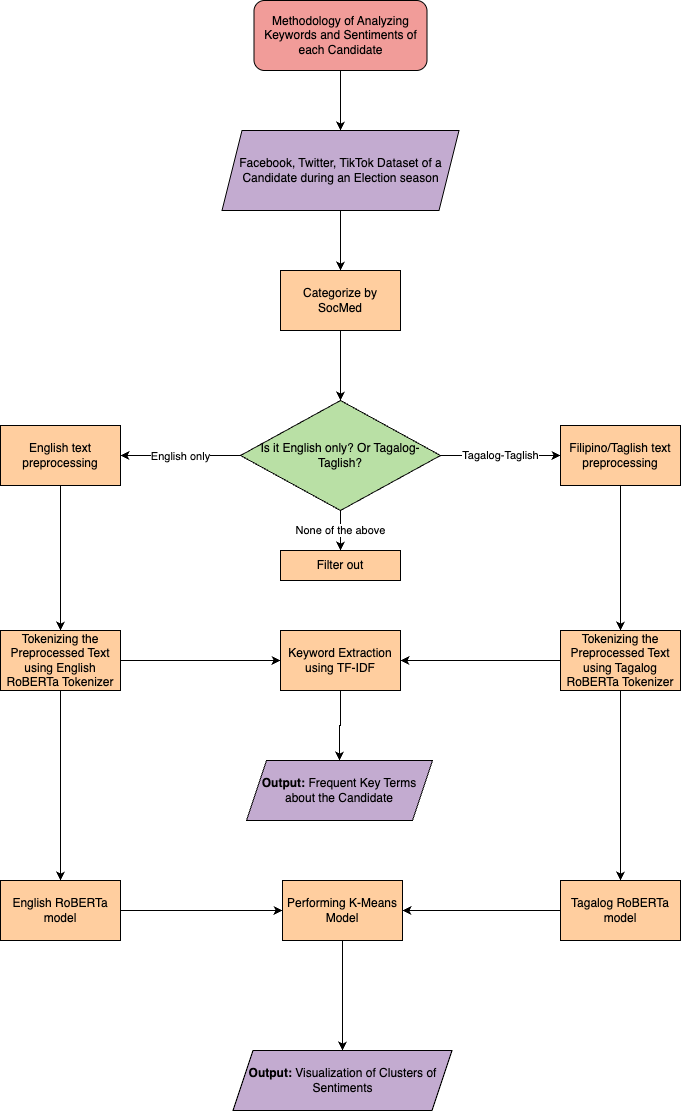
\includegraphics[width=1\textwidth]{Figures/methodology_flowchart.png}
    \caption{Methodology Flowchart}
    \label{fig:Methodology}
\end{figure}

% \clearpage

\section{Data Collection}
There are publicly available datasets for the 2024 US Presidential elections; however, for the 2022 Philippine Presidential Elections, the researchers will have to use a third-party Application Program Interface (API) due to the discontinued official free Academic API from X (former Twitter). In collecting tweets, keywords and dates will be utilized to perform an advanced search to get the tweets needed for the analysis.\newline

\begin{table}[h]
    \centering
    \begin{tabularx}{\textwidth}{X|X|X|X}
        \textbf{Presidential Election Year} & \textbf{Intention to Run Announcement} & \textbf{Dates within the Dataset (Inclusive)} & \textbf{Key Terms}\\
        \hline\hline
        \multirow{2}{*}{2022}& Marcos and Duterte: October 5, 2021 & \multirow{2}{*}{May 9, 2022} & \multirow{2}{4cm}{Marcos, Duterte, Robredo, Kiko, Pangilinan, BBM, Leni, DU30, Uniteam, Bongbong} \\
        & Robredo and Pangilinan: October 7, 2021 & & \\
    \end{tabularx}
    \caption{Table for Philippine Dataset Ranges}
\end{table}

\begin{table}[h]
    \centering
    \begin{tabularx}{\textwidth}{X|X|X|X}
        \textbf{Presidential Election Year} & \textbf{Intention to Run Announcement} & \textbf{Dates within the Dataset (Inclusive)} & \textbf{Key Terms}\\
        \hline\hline
        \multirow{2}{*}{2024}& Trump and Vance: November 15, 2022 & \multirow{2}{*}{November 8, 2024} & \multirow{2}{4cm}{Harris, Walz, Trump, Vance, Kamala, JD Vance} \\
        & Harris and Walz: July 21, 2024 & & \\
    \end{tabularx}
    \caption{Table for United States Dataset Ranges}
\end{table}

The end dates are until election day because of the high chances of a spike of sentiments especially as election days come closer.

Each collected tweet is in JSON format. For it to be utilized for natural language processing, it will be saved as a \texttt{.csv} file, separated, with each row marked by which country it belongs to, because it will be utilized for text classification.

\section{Data Preprocessing}
Before a group of datasets is fed into a tokenizer, they will undergo text processing.  Stop words such as \emph{“the,” “a,” “is”}, etc., will not be removed as they might be considered for the full context of a sentence when performing byte-tokenization. The following steps to preprocess the text will be as follows:

\begin{itemize}
    \item Omitting a tweet from the dataset if it is not in English, Tagalog, or a mix of them. The languages of the tweets will be detected by the Python library \texttt{langdetect}.
    \item Removing punctuation marks that have no significance for sentiment analysis.
    \item Replacing emojis with special tags.
    \item Removing unnecessary emojis or replacing emojis with special tags describing them if it is necessary for sentiment analysis.
    \item Lowercasing the text.
    \item Handling links and email addresses by replacing them with a placeholder.
    \item Removing whitespaces and replacing multiple spaces with a single space.
    \item Adding paddings to equalize the length of sentences.
\end{itemize}

The preprocessed dataset will be placed in a new \texttt{.csv} file. It is expected that the dataset, after they are preprocessed, will be 20,000 tweets per election.

\section{Text Classification and Visualization}
\subsection{XLM-RoBERTa}
After the preprocessing, the dataset will be fed into the following models: the \texttt{XLM-RoBERTa} model for contextualized embedding and the TF-IDF model for determining frequent keywords. XLM-RoBERTa’s language-agnostic approach makes it easier to implement as there is no need to identify if certain texts are in English or Tagalog.

Once the preprocessed dataset is fed into the model, the resulting tokens will be used to determine frequent keywords via TF-IDF and semantic similarities on the embedding model.

\subsection{GMM Model}
Once the embeddings are generated, they will be compared for semantic similarity via \texttt{Gausian Mixture Model (GMM)}, an unsupervised probabilistic clustering algorithm. GMM clustering, in contrast with K-Means clustering, are modelled as Gausian distributions, providing them flexbilitiy in handling overlapping clusters and variance differences, especially XLM-RoBERTa produces contextualized embeddings in high dimensions. In the context of nuanced tweets or tweets with mixed emotions, GMM’s soft clustering handles it better because it gives probability distributions, which is valuable for interpreting such tweets. The embeddings will be fed into the GMM model and it will provide soft assignments to each embedding, allowing them to belong to multiple clusters with different probabilities. The manually marked sentiments, which will be colored in the visualization, will serve as an evaluation to see if the tweets of same sentiments belong to the same clusters.

The clusters will be quantitatively evaluated by \texttt{Adjusted Rand Index\\(ARI)}, which examines the similarity between two clustering assignments. It will be used to determine if the agreement between the sentiment clusters and manually labelled sentiments.

% \subsection{K-Means Model}
% Once the embeddings are generated, they will be compared for semantic similarity via K-Means clustering. Since the model has a feature that helps determine if a tweet’s sentiment is positive, negative, or neutral, it will become a color indicator in the visualization of clusters to determine a cluster’s sentiment and visualize echo chambers. This will be crucial in comparing and contrasting the social media presence and activity of each candidate.

\subsection{TF-IDF}
Meanwhile, the tokenized texts will also go to the \texttt{TF-IDF model} to determine the frequency of words. The frequency of the words is sorted by how frequently they are used in a certain post or comment. The top keywords per candidate will be used to compare and contrast with other candidates and the social media spheres of the two countries.

\subsection{Visualization}
The interactive visualizations of the analysis consist of the following: a word cloud of the most frequent words and cluster visualization of semantic meanings. Using the time and date indicated in the dataset, they will be used to visualize the sentiments of the tweets during early election, mid-election, days before the election, and the election day itself. It will also highlight the surveys from public opinion polls to match if these strong sentiments has a correlation with the public polls and the election turnout on the day of election.
\begin{figure}[h]
    \centering
    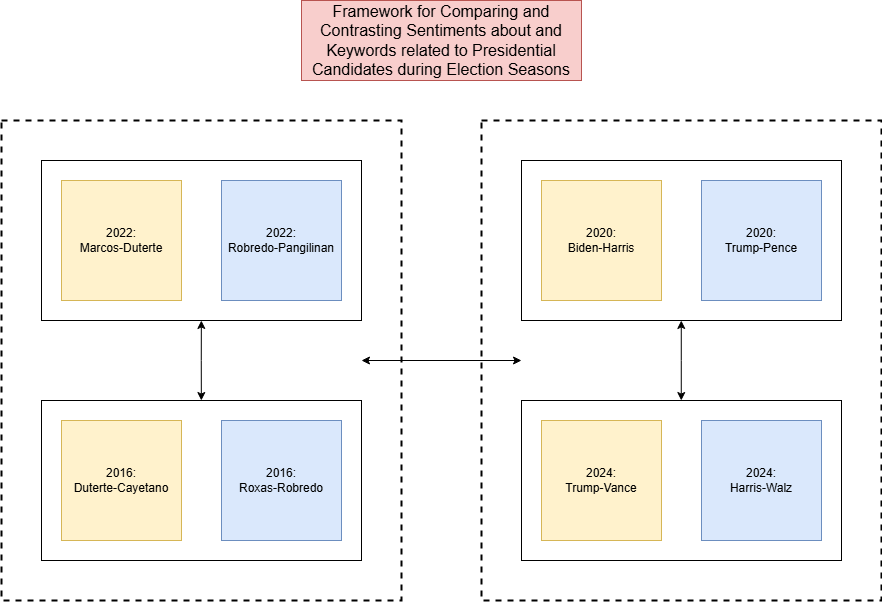
\includegraphics[width=0.65\textwidth]{Figures/methodology_framework-for-comparing.png}
    \caption{Framework for Comparing and Contrasting Sentiments}
    \label{fig:Framework-for-sentiments}
\end{figure}
% \chapter{RESULTS AND DISCUSSION}
% \section{Method of Measuring Accuracy of Approximated Coordinates}
% There were three methods used in the measuring of the accuracy of the approximated latitude and longitude coordinates produced by the discussed methodologies in this study. These three are: 1) looking at the Mean Absolute Error of the approximated coordinates compared to the actual coordinates of the tweets in the dataset, 2) using the Haversine Formula to get the average distance of each approximated coordinate from its actual location, and 3) using the Vincety Formula in place of the Haversine Formula. It is to be noted that the LDA-LSA Double Filter (first methodology) used only half of the dataset as test data while the Dynamic Dictionaries Per Region method (second methodology) used the entire dataset. 

% \subsection{Mean Absolute Error}
% Python's Scikit-Learn library was used in measuring the Mean Absolute Error of the approximated coordinates versus the actual coordinates for both methodologies. The Mean Absolute Error value is a measure which determines the error of all the given values in a dataset relative to another set. The best possible result for a Mean Absolute Error score is 0 since this indicates that there is no disparity between any of the compared values.

% The Mean Absolute Error scores for both methodologies are found in \ref{tab:acc_lit}.

% \begin {table*}[h]
% \centering
% \caption {\textbf{Mean Absolute Error Scores of Methodologies}}
% \label{tab:acc_lit} 
% \begin{tabular}{ c  c  c  c }
% \hline
% Methodology	&Latitude  	&Longitude 	&Average \\
% Type  &MAE   &MAE   &MAE   \\
%    \hline

% LDA-LSA  &1.66  &1.07  &1.36  \\
% Dynamic Dicts. &2.02   &1.30   &1.66   \\  \hline
% \end{tabular}
% \end{table*}

% \subsection{Haversine Formula}
% The Haversine Formula is a trigonometric method of measuring the distance of two coordinates. This way of measurement assumes that the two points being measured against one another belongs in a spherical space. 

% The results of applying the Haversine Formula to measure the distance of each approximated coordinate versus its actual coordinates are shown in Table 4.2.

% \begin {table*}[h]
% \centering
% \caption {Haversine Formula Scores of Methodologies}
% \label{tab:acc_lit2} 
% \begin{tabular}{ c  c  }
% \hline
% Methodology	&Average Haversine   \\
% Type  &Distance (in KM)     \\
%    \hline

% LDA-LSA  &223.94    \\
% Dynamic Dicts. &271.71    \\  \hline
% \end{tabular}
% \end{table*}

% \subsection{Vincenty Formula}
% The Vincenty Formula functions in a similar way as the Haversine Formula. The only difference is that the Vincenty Formula is a more widely-used method of computation in GPS devices. In principle, the Vincenty Formula uses the same trigonometric principles of computing the distances between two coordinates in a spherical space.

% The results of the Vincenty Formula on the two methodologies is shown in Table 4.3.

% \begin {table*}[h]
% \centering
% \caption {Vincenty Formula Scores of Methodologies}
% \label{tab:acc_lit3} 
% \begin{tabular}{ c  c  }
% \hline
% Methodology	&Average Vincenty \\
% Type  &Distance (in KM)   \\
%    \hline

% LDA-LSA  &223.15  \\
% Dynamic Dicts. &270.75      \\  \hline
% \end{tabular}
% \end{table*}

% \section{Visualization of Results}
% This section tackles the visualization of the results of both methodologies. Geolocated tweets were grouped into clusters for the purpose of visualization. The geolocated tweets from the first methodology were clustered based on topics, while the tweets from the second methodology were clustered based on geographic region. 


% \begin{figure}
%     \centering
%     \includegraphics[width=\textwidth, height=\textheight,keepaspectratio]{Method1OrigMap.png}
%     \caption{LDA-LSA Double Filter Plot of Original Tweets}
%     \label{fig:my_label1}
% \end{figure}

% \begin{figure}
%     \centering
%     \includegraphics[width=\textwidth, height=\textheight,keepaspectratio]{Method1ApproxMap.png}
%     \caption{LDA-LSA Double Filter Plot of Approximated Tweets}
%     \label{fig:my_label2}
% \end{figure}

% \begin{figure}
%     \centering
%     \includegraphics[width=\textwidth, height=\textheight,keepaspectratio]{Method1Cluster1.PNG}
%     \caption{LDA-LSA Double Filter Clusters 1-3}
%     \label{fig:my_label3}
% \end{figure}


% \begin{figure}
%     \centering
%     \includegraphics[width=\textwidth, height=\textheight,keepaspectratio]{Method1Cluster2.PNG}
%     \caption{LDA-LSA Double Filter Clusters 4-6}
%     \label{fig:my_label4}
% \end{figure}

% \begin{figure}
%     \centering
%     \includegraphics[width=\textwidth, height=\textheight,keepaspectratio]{Method1Cluster3.PNG}
%     \caption{LDA-LSA Double Filter Clusters 7-9}
%     \label{fig:my_label5}
% \end{figure}

% \begin{figure}
%     \centering
%     \includegraphics[width=\textwidth, height=\textheight,keepaspectratio]{Method1Cluster4.PNG}
%     \caption{LDA-LSA Double Filter Cluster 10}
%     \label{fig:my_label6}
% \end{figure}

% \begin{figure}
%     \centering
%     \includegraphics[width=\textwidth, height=\textheight,keepaspectratio]{Method2OrigMap.png}
%     \caption{Dynamic Dictionaries Per Region Plot of Original Tweets}
%     \label{fig:my_label7}
% \end{figure}

% \begin{figure}
%     \centering
%     \includegraphics[width=\textwidth, height=\textheight,keepaspectratio]{Method2ApproxMap.png}
%     \caption{Dynamic Dictionaries Per Region Plot of Approximated Tweets}
%     \label{fig:my_label8}
% \end{figure}

% \begin{figure}
%     \centering
%     \includegraphics[width=\textwidth, height=\textheight,keepaspectratio]{Method2Cluster.PNG}
%     \caption{Dynamic Dictionaries Per Region Clusters}
%     \label{fig:my_label9}
% \end{figure}

% \subsection{LDA-LSA Double Filter Visualized Results}
% Figure \ref{fig:my_label1} to \ref{fig:my_label6} shows the plots and cluster legend for the results of the first methodology. Figure \ref{fig:my_label1} shows that the original tweets that were clustered into the same topics were not necessarily within close geographic proximity among each other. In the case of some clusters, there were tweets that belonged in different parts of the Philippines. For example, there were tweets in Luzon and in Mindanao that were classified to the same cluster of topics. 

% Figure \ref{fig:my_label2} shows the plot for the first methodology's geolocated tweets. As seen in the figure, the tweets belonging in the same cluster are more geographically clumped up together in general. It may be noted that the majority of the tweets were approximated to be located near the Visayas region and south of the NCR. It is also apparent that there are groups of tweets that were geolocated in invalid locations such as bodies of water. 

% Figures \ref{fig:my_label3} to \ref{fig:my_label6} serve as the legend of clusters for Figures \ref{fig:my_label1} and \ref{fig:my_label2}. There were ten clusters used for the LDA-LSA Double Filter methodology. Each cluster contains ten topics in string form with similar themes. The ten clusters used reflect the number of topics that were used to train the LDA model as discussed in the methodology section. The color for each cluster of topics are also specified. 

% \subsection{Dynamic Dictionaries Per Region Visualized Results}
% Figures \ref{fig:my_label7} to \ref{fig:my_label9} display the plots and cluster legend for the Dynamic Dictionaries Per Region methodology. Figure \ref{fig:my_label7} contains the plot of the original tweets from the dataset used in this study. It may be observed that all Philippine geographic regions contain at least one tweet in their vicinity, with a majority of them being located in Central Luzon. 

% Figure \ref{fig:my_label8} is the plot of the geolocated tweets from the Dynamic Dictionaries Per Region methodology algorithm. There are some Philippine geographic regions shown in Figure \ref{fig:my_label8} that do not contain any tweets unlike in Figure \ref{fig:my_label7}. It is also worth noting that there were groups of tweets that were geolocated in bodies of water similar to the case of the LDA-LSA Double Filter methodology. Lastly, Figure \ref{fig:my_label9} shows the legend of clusters for the Dynamic Dictionaries Per Region methdology.

% All plots and figures were created via Python scripts. Any program that has Python support may recreate these plots accordingly. 

% \section{Insights}
% The results of both methodologies provide several insights. It appears that the first methodology (LDA-LSA Double Filter) outperformed the second (Dynamic Dictionaries Per Region) in all three metrics used to measure the accuracy of the results of both.

% The closer to zero the Mean Absolute Error of a dataset is compared to another, the better. Again, a value of 0 indicates that the values of a test dataset completely matches that of the values of a given target dataset. The Mean Absolute Error value of the first methodology is lower by 0.3 compared to the second. This means that the approximated coordinates from the first methodology are closer to the actual coordinates in the dataset than the ones from the second.

% The Haversine Formula and Vincenty Formula results show a similar trend. The first methodology's scores are significantly better than the second's for both metrics. This indicates that the approximated coordinates from the first methodology are nearer to their actual coordinates from dataset in terms of kilometers. This means that given these results, it is more effective to approximate a given disaster-related tweet according to the topic it belongs to than its geographic region. 

% A possible reason as to why the second methodology yielded worse results is because there are some Philippine regions that cover relative large geographic areas. This means that it is possible that the approximated latitude and longitude coordinates of a given tweet belongs in the same region as its original coordinates, but not necessarily in the same vicinity. Some areas within certain Philippine regions are separated by tens or even hundreds of kilometers. This may contribute to high distance disparity between the actual and approximated values. This is perhaps the main drawback of classifying tweets per region. 

% Another possible reason as to why the first methodology outperformed the second is the structure of the dataset that was used in this study. It was found that over sixty percent of the tweets in the dataset belonged in the NCR and that some regions contained anywhere from nine to twenty-five tweets only. This may cause the execution of the second methodology to perform worse because the models representative of all geographic regions are not equally refined/trained. There are some models that are more refined than others since the number of tweets are not equally distributed across all available regions. This conversely means that some models are poorly trained because there are only several tweets from that region as far as the dataset used is concerned. The differences in refinement of the geographic models may cause the models to classify a given query tweet to the incorrect region because it is more likely that the more refined models will be selected by the algorithm described in the previous sections. The richer models have more depth in terms of stored information and thus are more capable of processing and identifying incoming query tweets as part of the geographic region they represent. It is highly likely that there are many cases where, for example, a tweet originally from the ARMM region may be recognized and classified as a tweet from the NCR since the model representative of the latter region is much better trained. This kind of scenario becomes increasingly likely to happen as the algorithm executes because the models refresh periodically after processing a certain number of tweets. The better trained models will be continuously further trained and refined as they process more tweets.

% These results however do not discount the fact that both methodologies still performed better than previous studies did as far as the Typhoon Yolanda tweets are concerned. An over 200 kilometer distance is still large, but this is a significant improvement from the findings of the previous studies discussed in the theoretical background section of this paper. The said previous studies had results of over 300 kilometers of distance for the approximated coordinates. Both methodologies had below 300 kilometers, which is a slight improvement. But again, the results indicate that while both methodologies are possible steps towards the right direction, the first methodology appears to be the more optimal approach for this dataset. It is also worth noting that the results of both methodologies showed that there were still quite a number of tweets that were geolocated in invalid locations such as bodies of water. Again, this is reflective of the fact that the Philippines is an archipelago, and that both methodologies may still be improved tremendously. 
% %\input{04_results_pub}
% %\input{04_results_unpub}
% \chapter{CONCLUSIONS}


%Upon presenting your results, the conclusion is where you will now %tie up these results with the original intent of the study, as %indicated by the research questions given in the Introduction. It is %in this section where you will also discuss any difficulties or %issues encountered during the study, as well as your recommended %method for addressing these problems.

%The general way to organize your conclusion is to present each %research sub-question as a subsection, and thoroughly answer each of %them by interpreting your results with respect to the question. With %these answered, you may then tie up all of your findings in each %subsection to answer your main research question, providing any %needed additional information or explanation. Last on the list would %be your unsolved issues and difficulties, presenting them as avenues %to motivate continued work on your chosen topic.
 
% \chapter{RECOMMENDATIONS}

% %\input{08_appendices_b_thesisformattingguidelines}

% % BIBLIOGRAPHY
\bibliographystyle{acm}

\bibliography{sigproc}
% \input{09_references}

% \BackMatter
% \bibliography{Proposal_Manuscript}
% \addappheadtotoc
% \begin{appendices}
%     \chapter{Methodology 1}

% \begin{figure}[htb]
%     \centering
%     \includegraphics[width=1\textwidth]{rrl_system-architecture.png}
%     \caption{System Architecture}
%     \label{fig:rrl_system-architecture}
% \end{figure}
%     \chapter{Methodology 2}

\begin{figure}[htb]
    \centering
    \includegraphics[width=1\textwidth]{Figures/rrl_system-architecture.png}
    \caption{System Architecture}
    \label{fig:rrl_system-architecture}
\end{figure}
% \end{appendices}


\end{document}